%--------------------------------------------------------------------
%--------------------------------------------------------------------
% Formato para los talleres del curso de Métodos Computacionales
% Universidad de los Andes
%--------------------------------------------------------------------
%--------------------------------------------------------------------

\documentclass[11pt,letterpaper]{exam}
\usepackage[utf8]{inputenc}
\usepackage[spanish]{babel}
\usepackage{graphicx}
\usepackage{tabularx}
\usepackage[absolute]{textpos} % Para poner una imagen en posiciones arbitrarias
\usepackage{multirow}
\usepackage{float}
\usepackage{hyperref}
%\decimalpoint

\begin{document}
\begin{center}
{\Large Métodos Computacionales} \\
\textsc{Tarea 2}\\
01-2019\\
\end{center}

\noindent
\section{Ejercicio 2: Transformada de Fourier}
\begin{center}
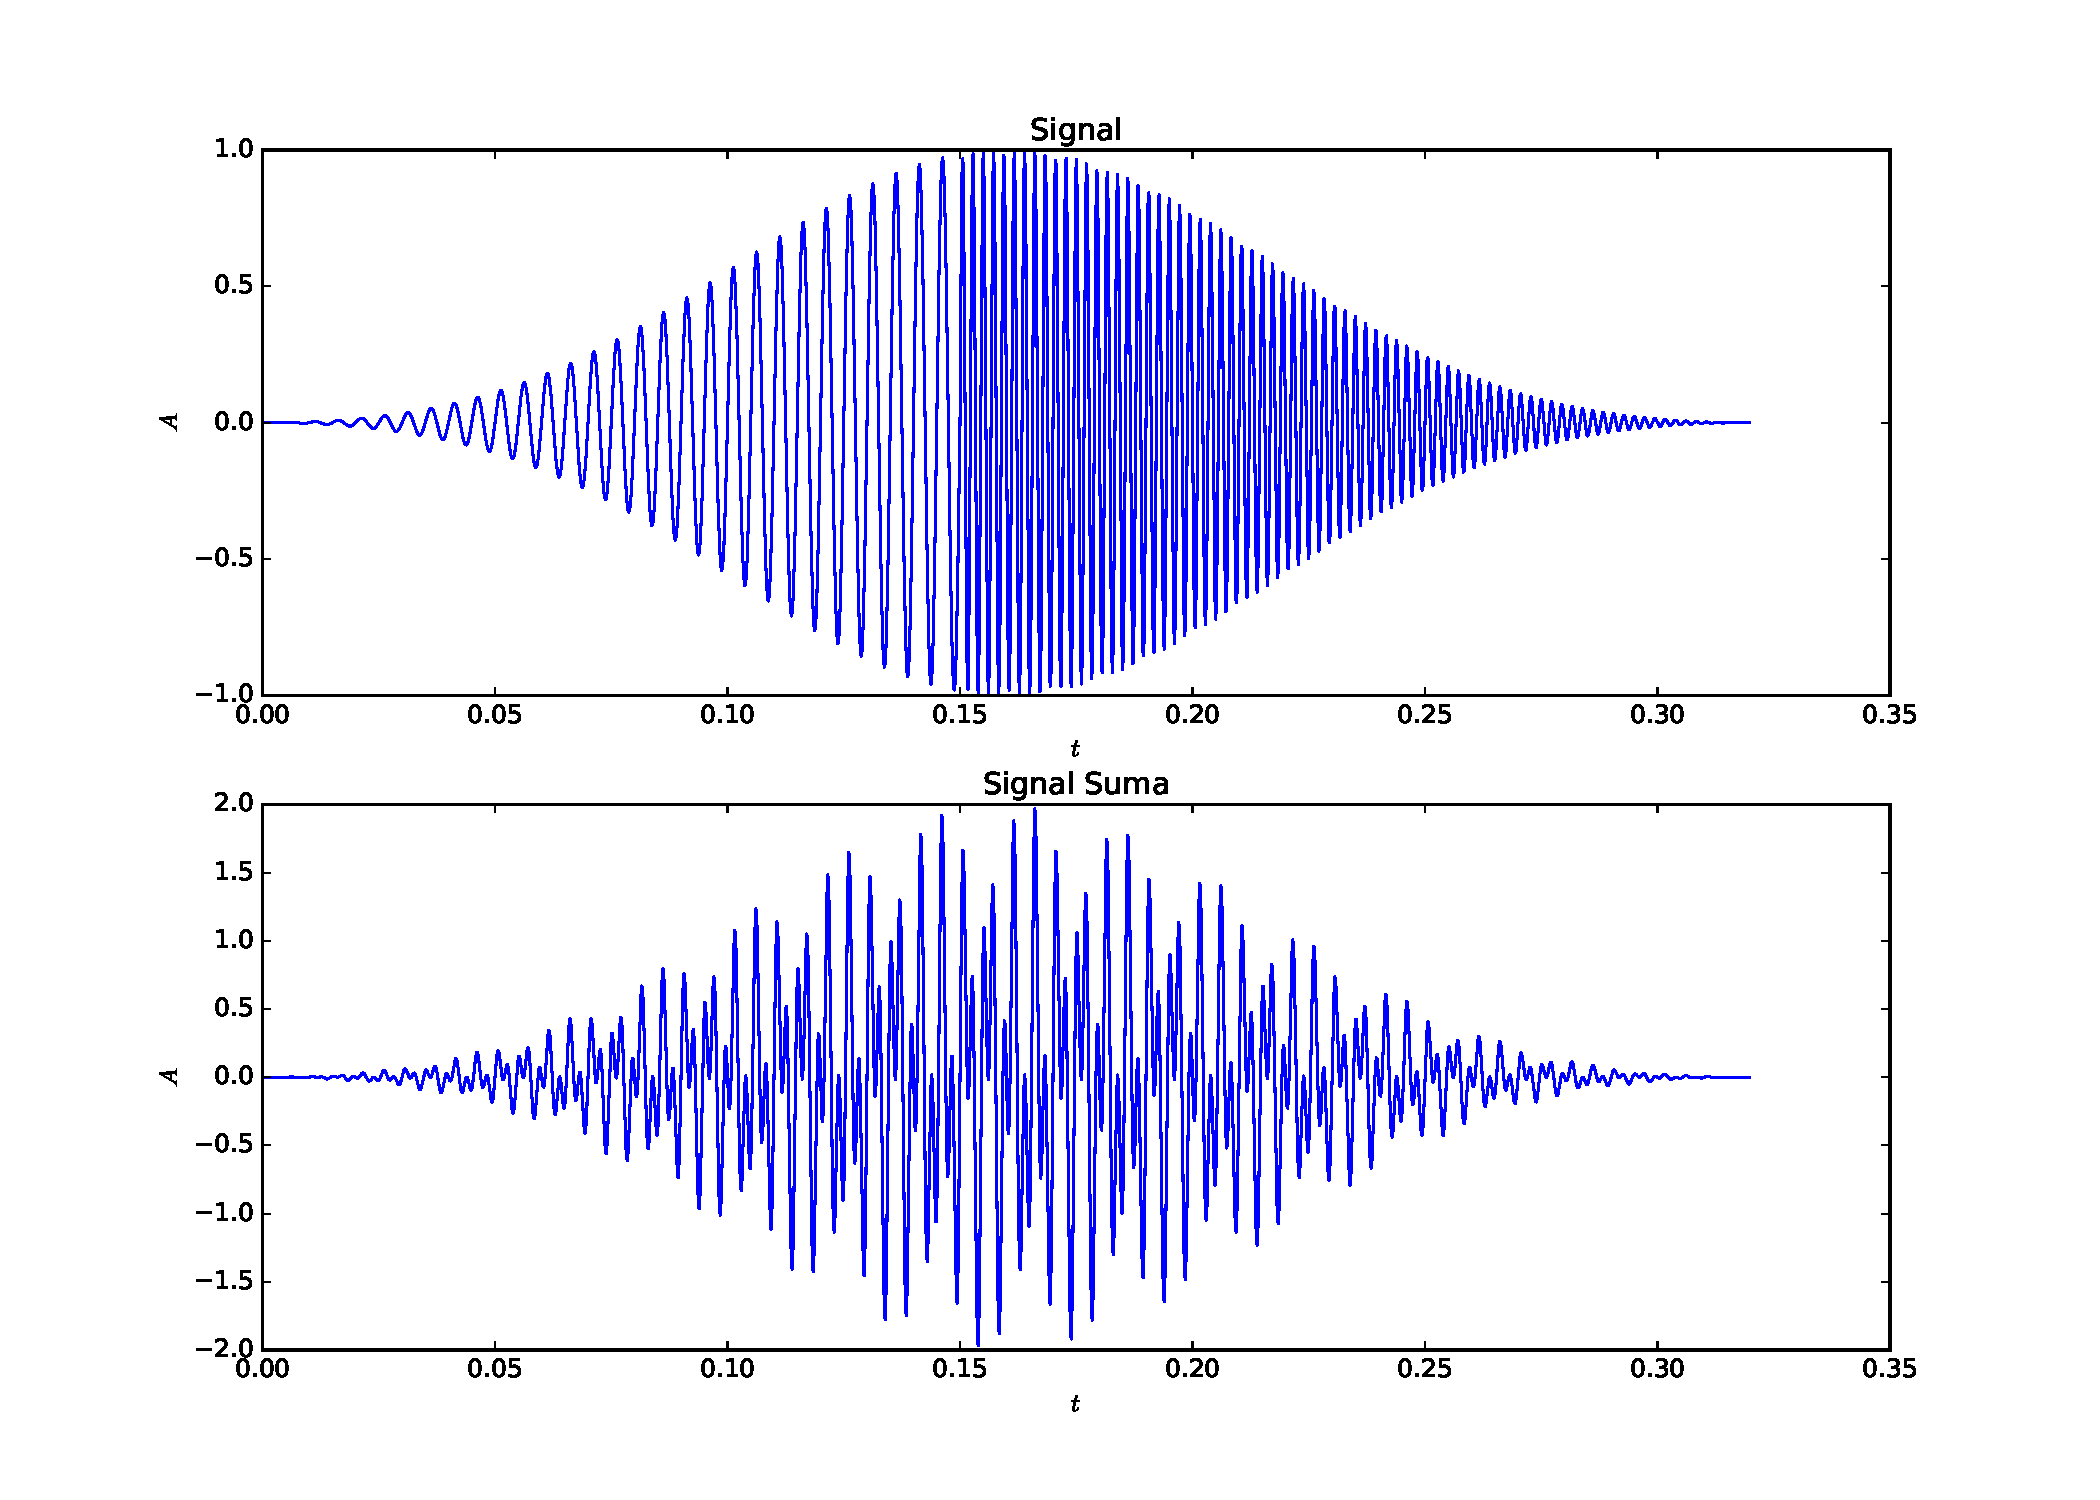
\includegraphics[width=14cm]{2_Signal.pdf} 
\end{center}
{Gráficas de las señales 'Signal' y 'SignalSuma'. Cualitativamente podemos ver que 'Signal' cambia de frecuencia 'principal' en $t=0.15$, mientras que 'SignalSuma' es la suma de dos señales con frecuencias distintas. } 
\begin{center}
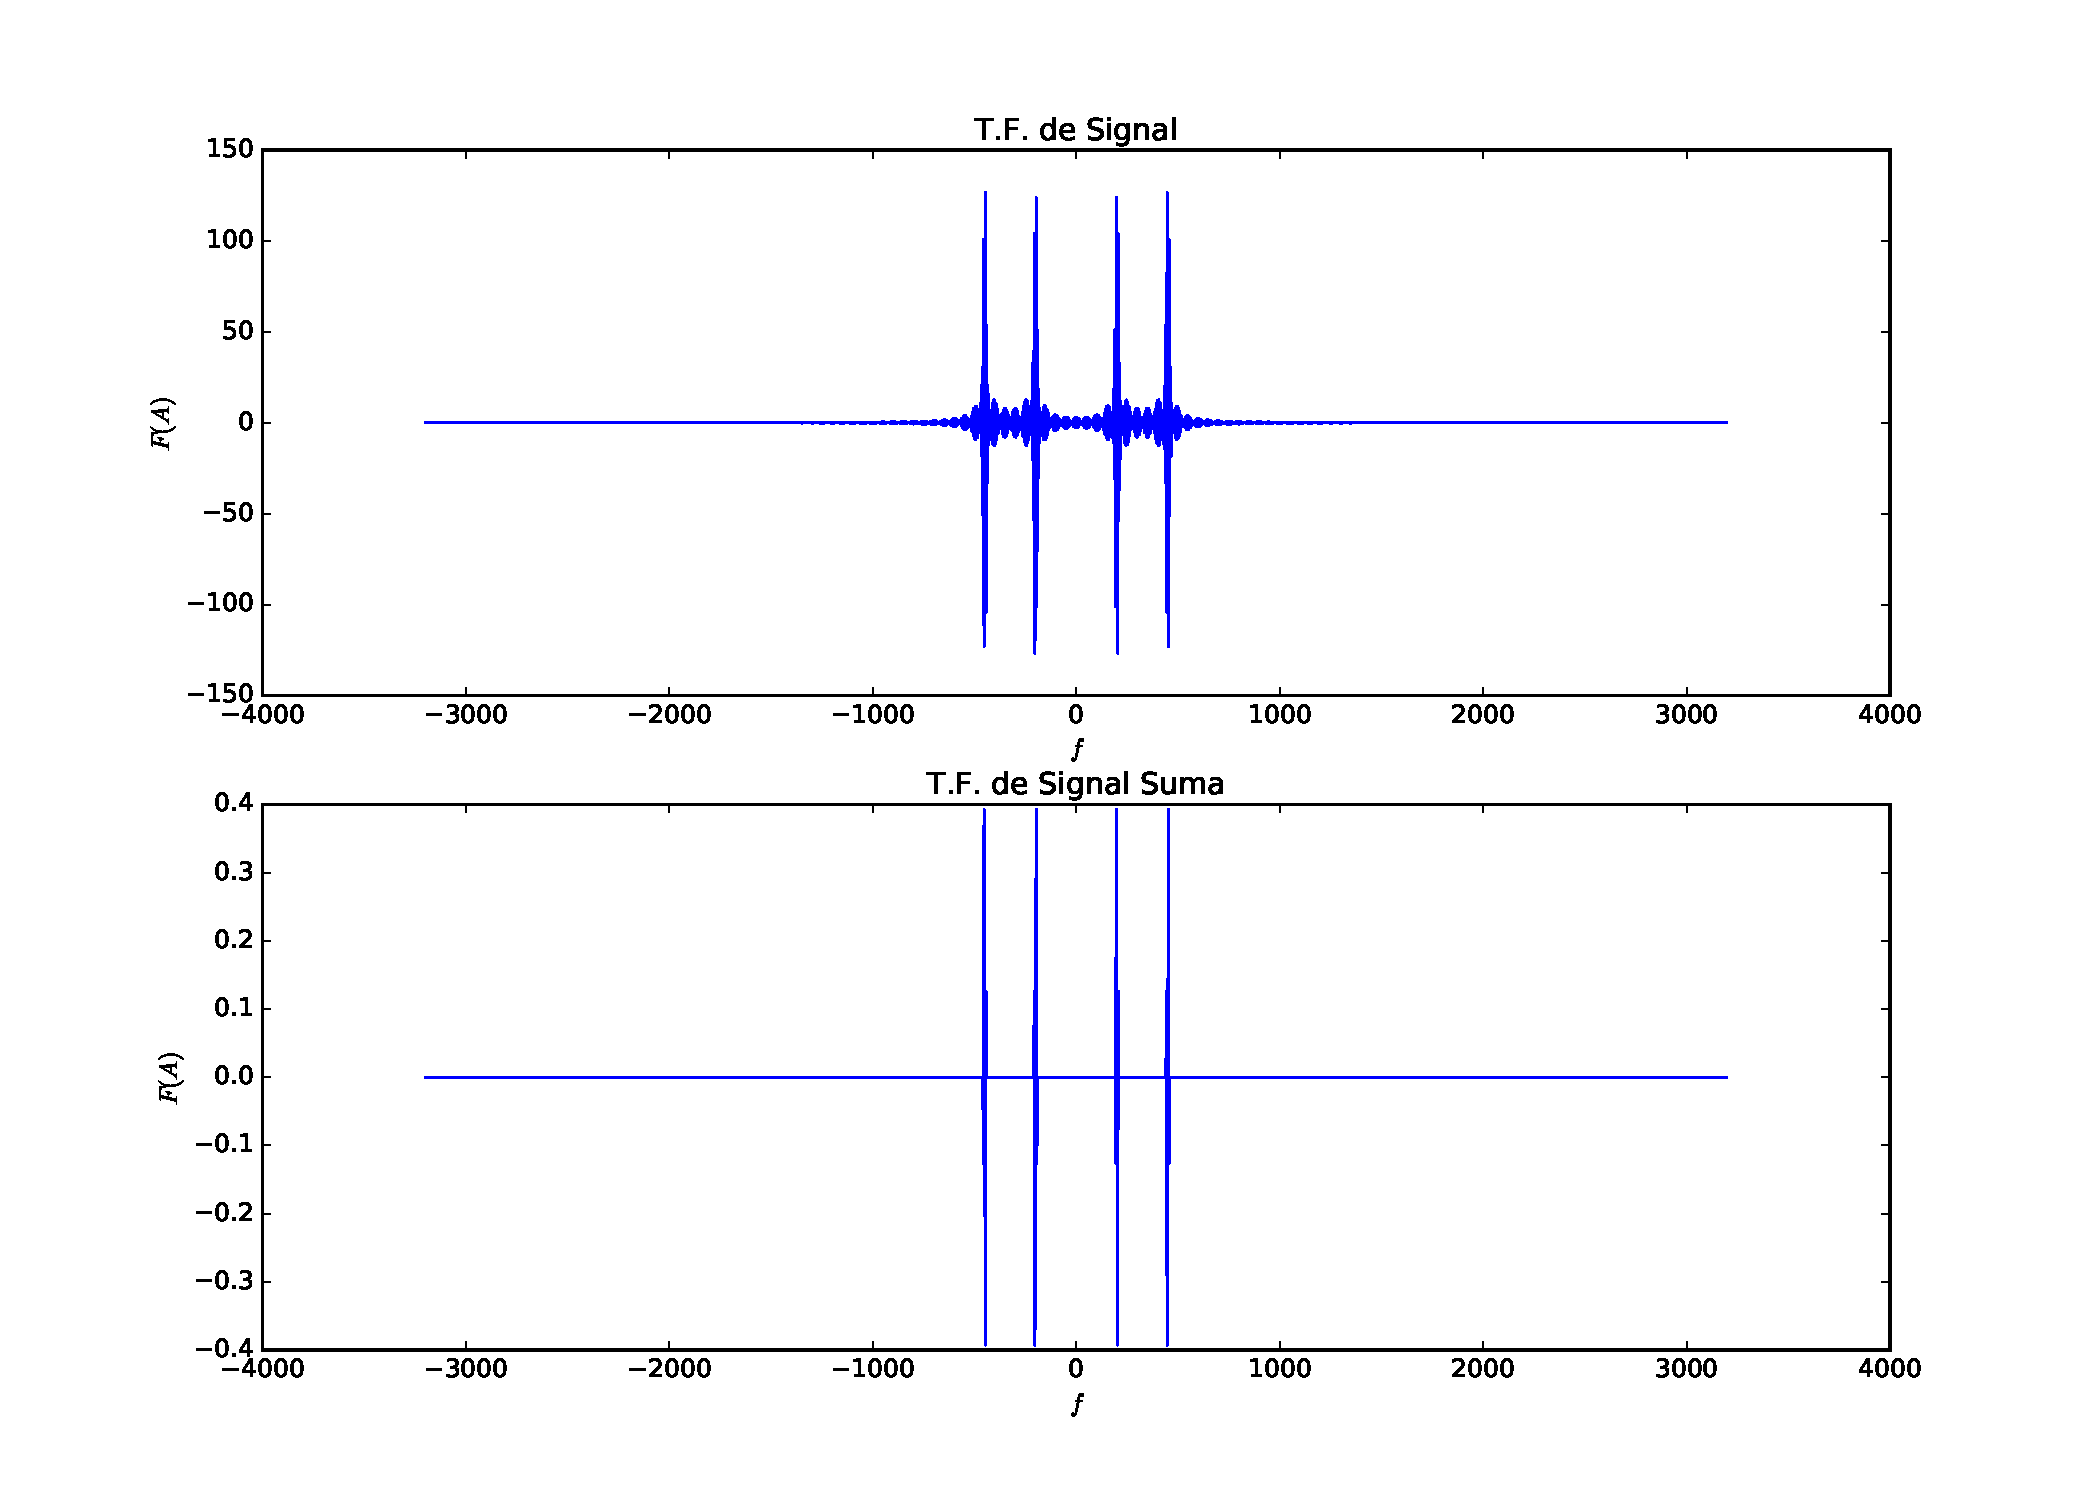
\includegraphics[width=14cm]{2_FourierSignal.pdf} 
\end{center}
{Transformadas de Fourier de 'Signal' y 'SignalSuma'. Aqu\'i es claro que Signal se compone de dos frecuencias principales $\sim \pm 200, \pm 400$, pero hay ciertas frecuencias intermedias que realizan el cambio que hemos mencionado. Por otro lado, SignalSuma sólo se compone de la superposición de dos frecuencias $\sim \pm 200, \pm 400$.}
\begin{center}
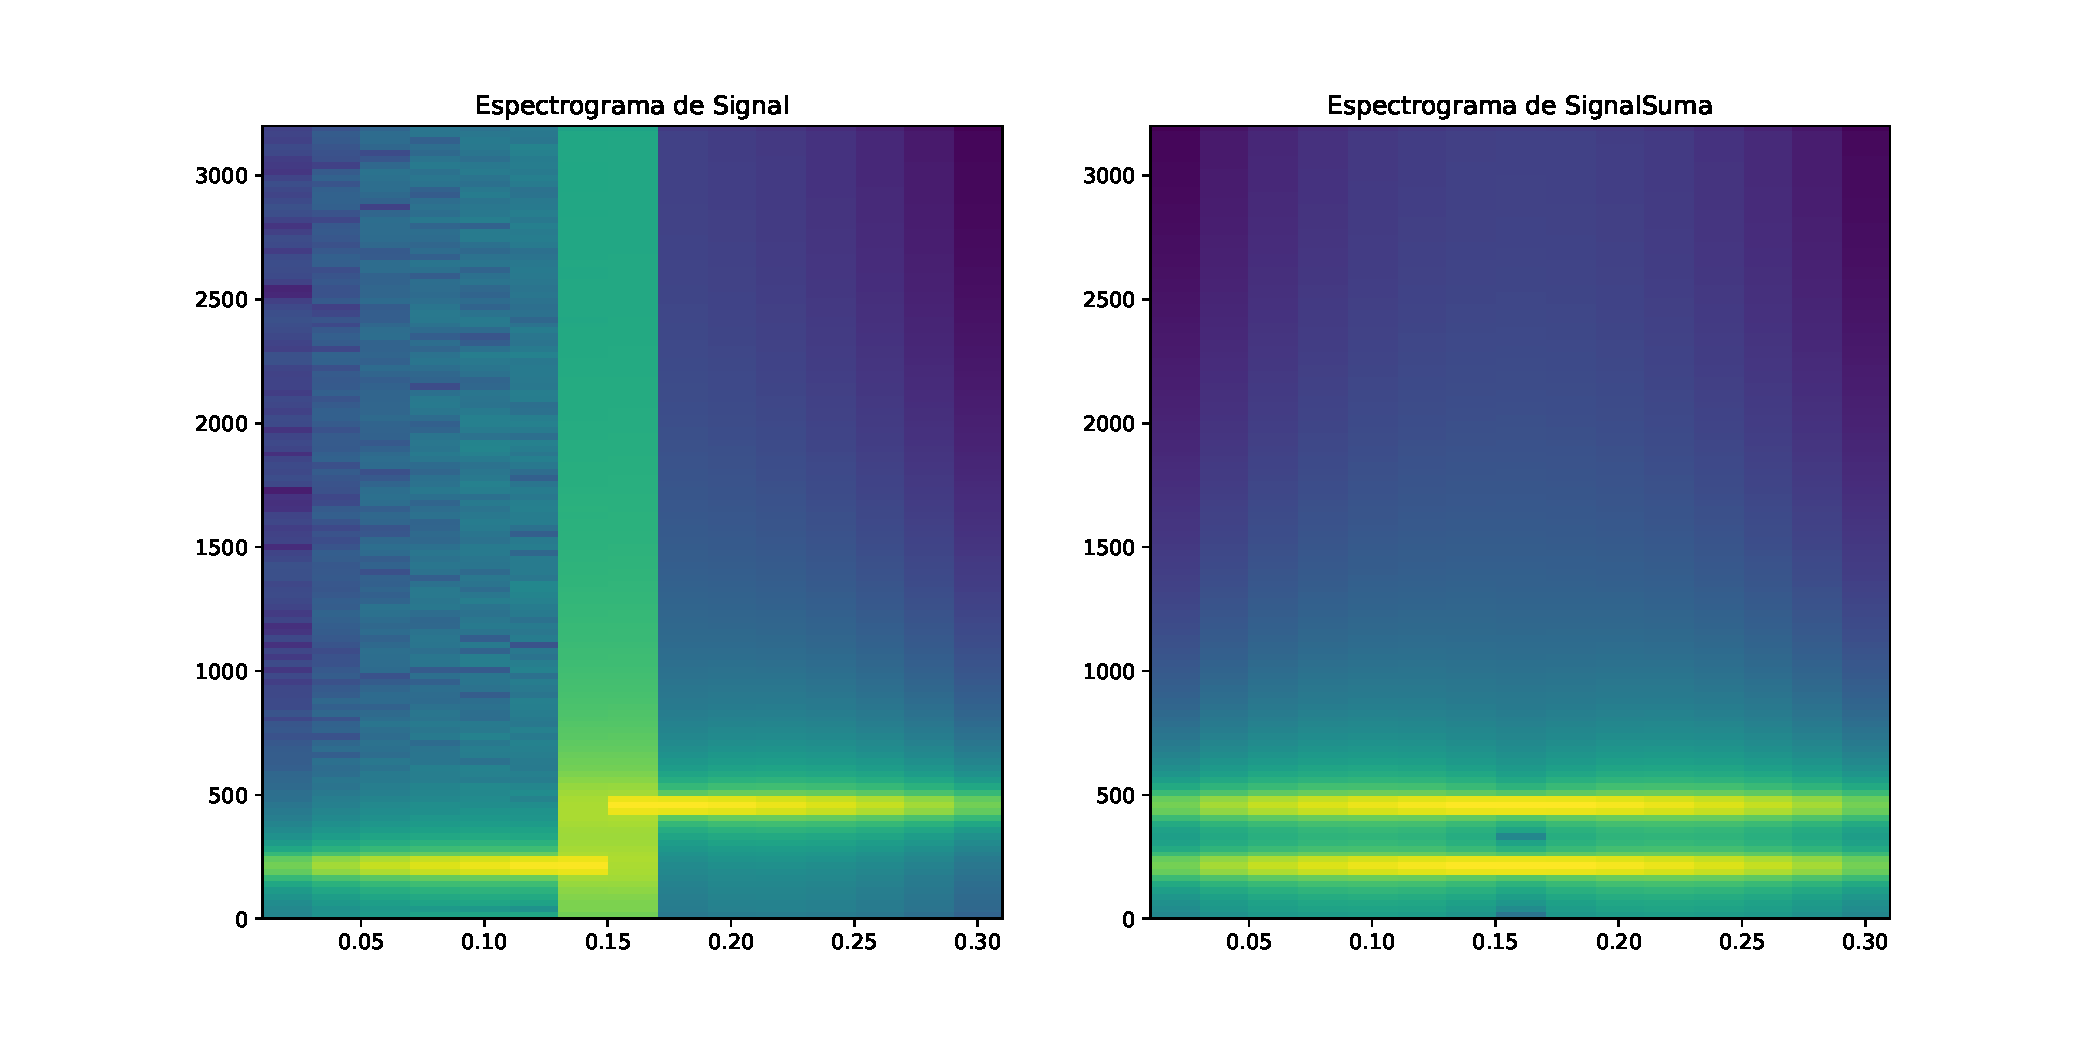
\includegraphics[width=14cm]{2_Espectrogramas.pdf} 
\end{center}
{Espectrogramas de Signal y SignalSuma. El espectrograma mapea la intensidad de cada una de las frecuencias individuales en cada momento $t$. Para Signal se ve la transici\'on de $\sim 200$ a $\sim 400$ alrededor de 0.15, donde tiene una breve superposición de ambas. Por otro lado, para SignalSuma es claro que las dos frecuencias que la componen están superpuestas en todo momento, como esper\'abamos.}
\begin{center}
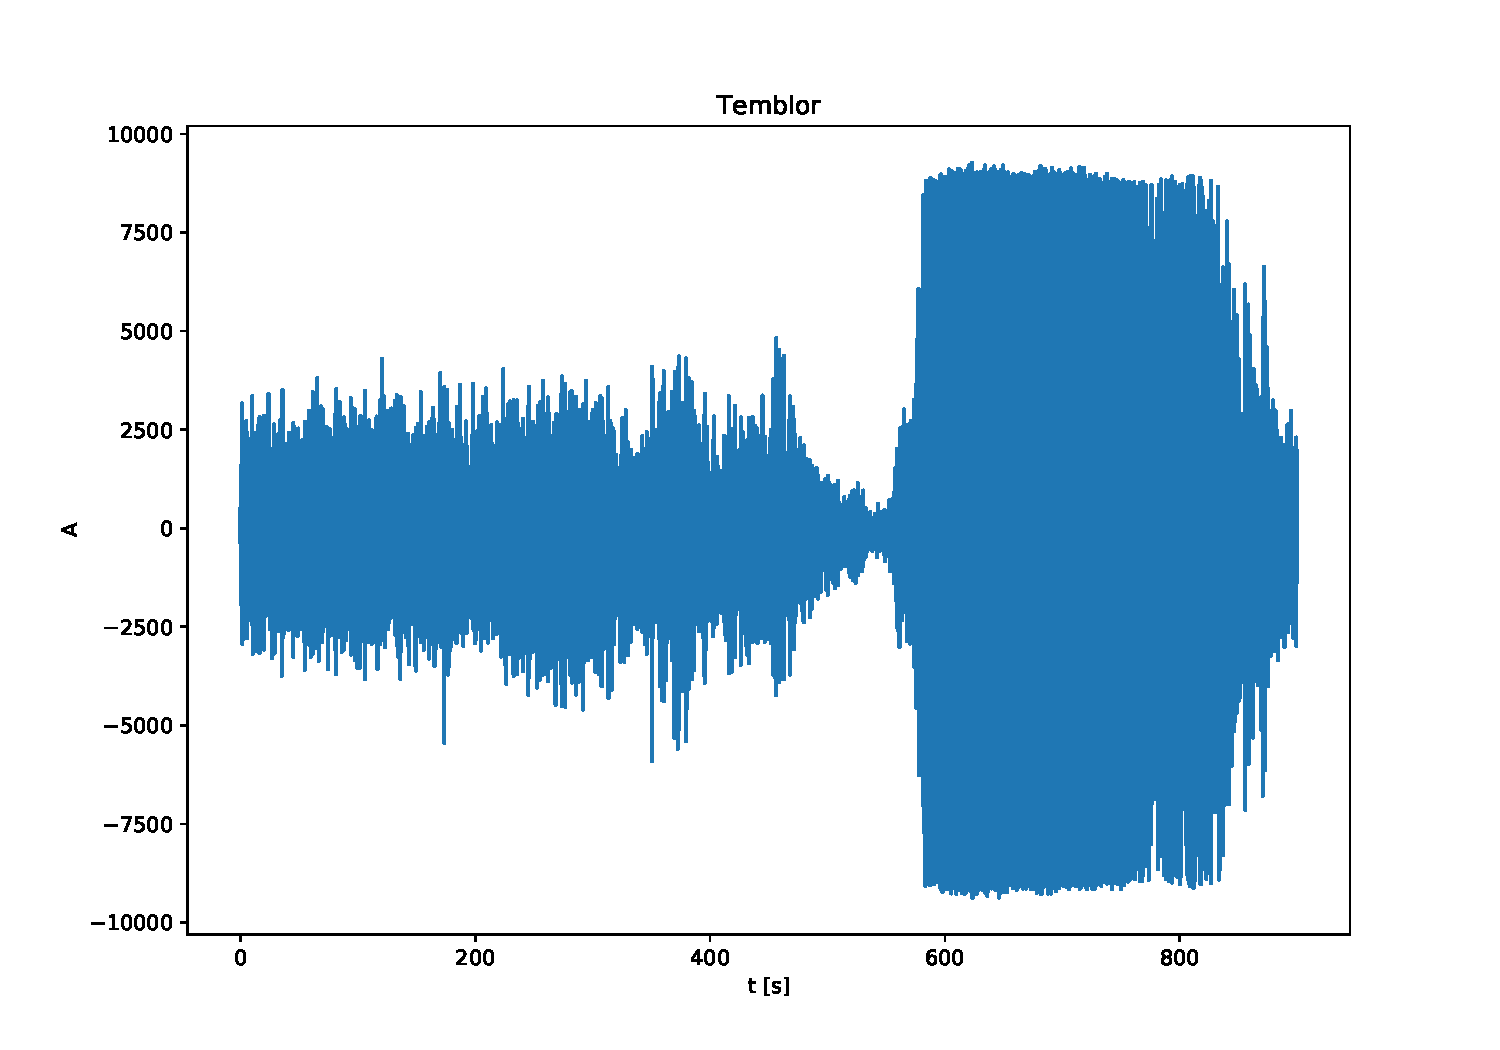
\includegraphics[width=14cm]{2_Temblor.pdf} 
\end{center}
{Gráfica de la señal del temblor. En principio no es muy claro de qué frencuencias se compone.}
\begin{center}
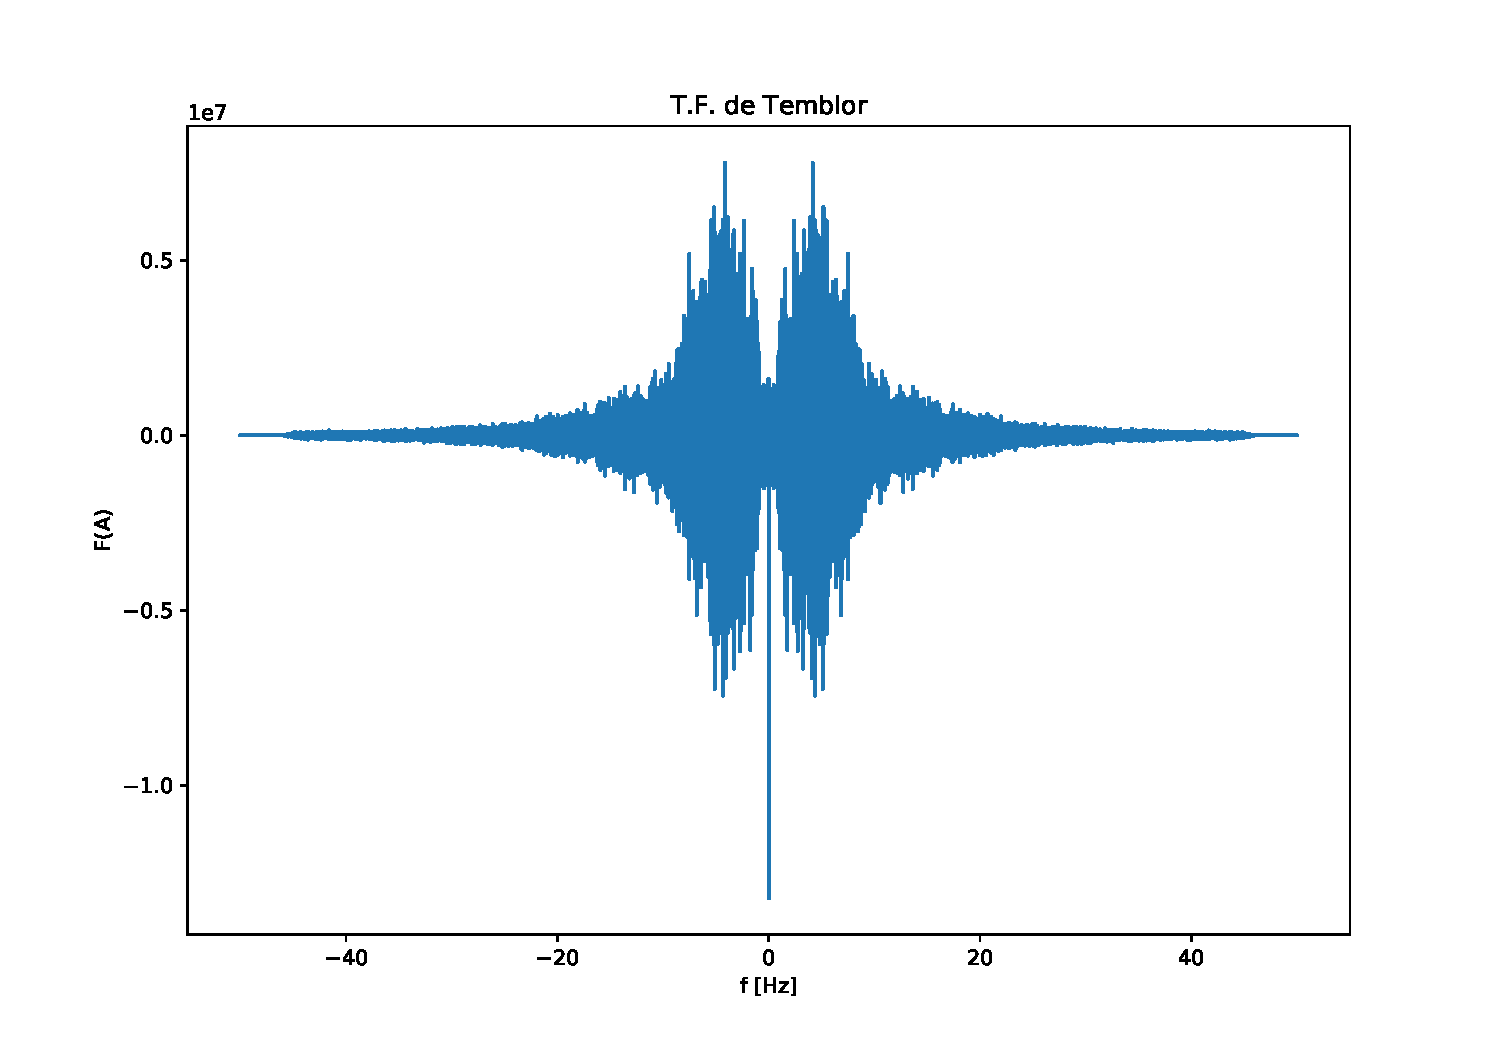
\includegraphics[width=14cm]{2_FourierTemblor.pdf}
\end{center}
{Transformada de Fourier del temblor. Acá se puede ver que hay una concentración de frecuencias alrededor de $\sim\pm 5 Hz$, la cual disminuye hacia frecuencias más altas, pero comienza repentinamente alrededor de $\sim\pm 1 Hz$. Esto concuerda con las frecuencias esperadas de ondas sísmicas, siendo relativamente 'bajas'. }
\begin{center}
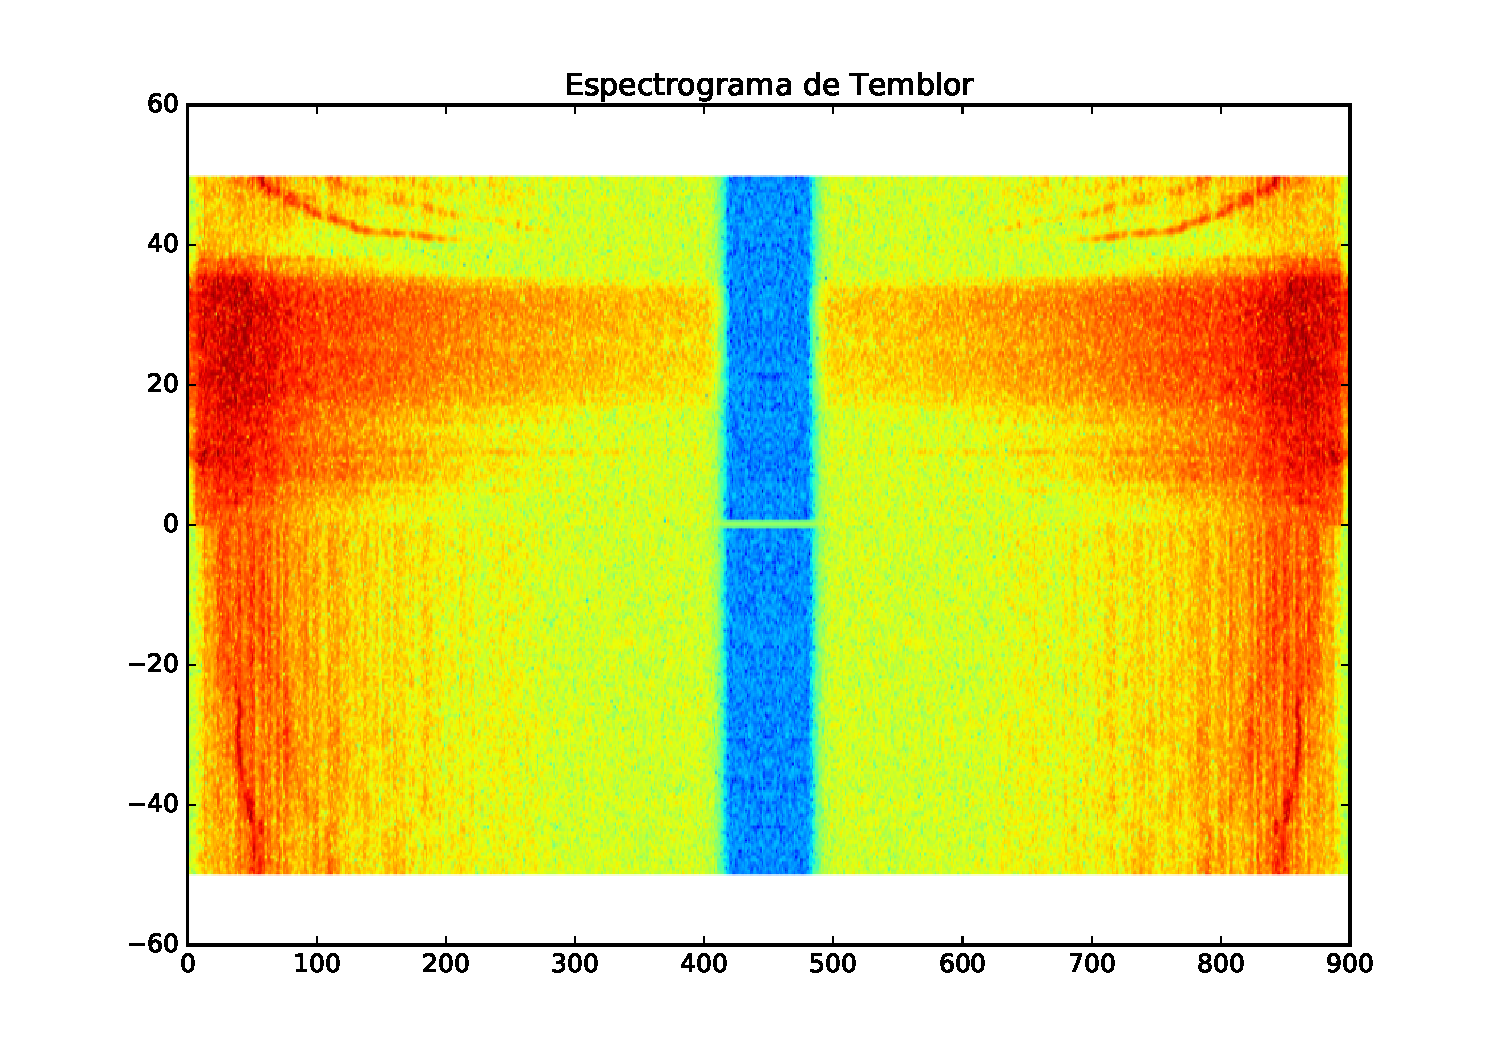
\includegraphics[width=14cm]{2_EspectrogramaTemblor.pdf}
\end{center}
Espectrograma del temblor. Acá se esclarece lo visto en la T.F. del temblor. Empieza teniendo una frecuencia baja $\sim 5 Hz$ la cual asciende rápidamente hasta un máximo $\sim 25 Hz$. De ahí en adelante hay una gran presencia de frecuencias alrededor de $\sim 5 Hz$. De hecho, esto concuerda con el análisis se hizo de este temblor en \texttt{https://www.sciencedirect.com/science/article/abs/pii/S0377027312000029}. Esta gráfica nos permite ver la utilidad del espectrograma, pues podemos identificar el comportamiento del temblor como una señal periódica a lo largo del tiempo, a diferencia de la T.F. únicamente. 

\section{Ejercicio 3: Ecuaciones diferenciales - edificio en un sismo}
\begin{center}
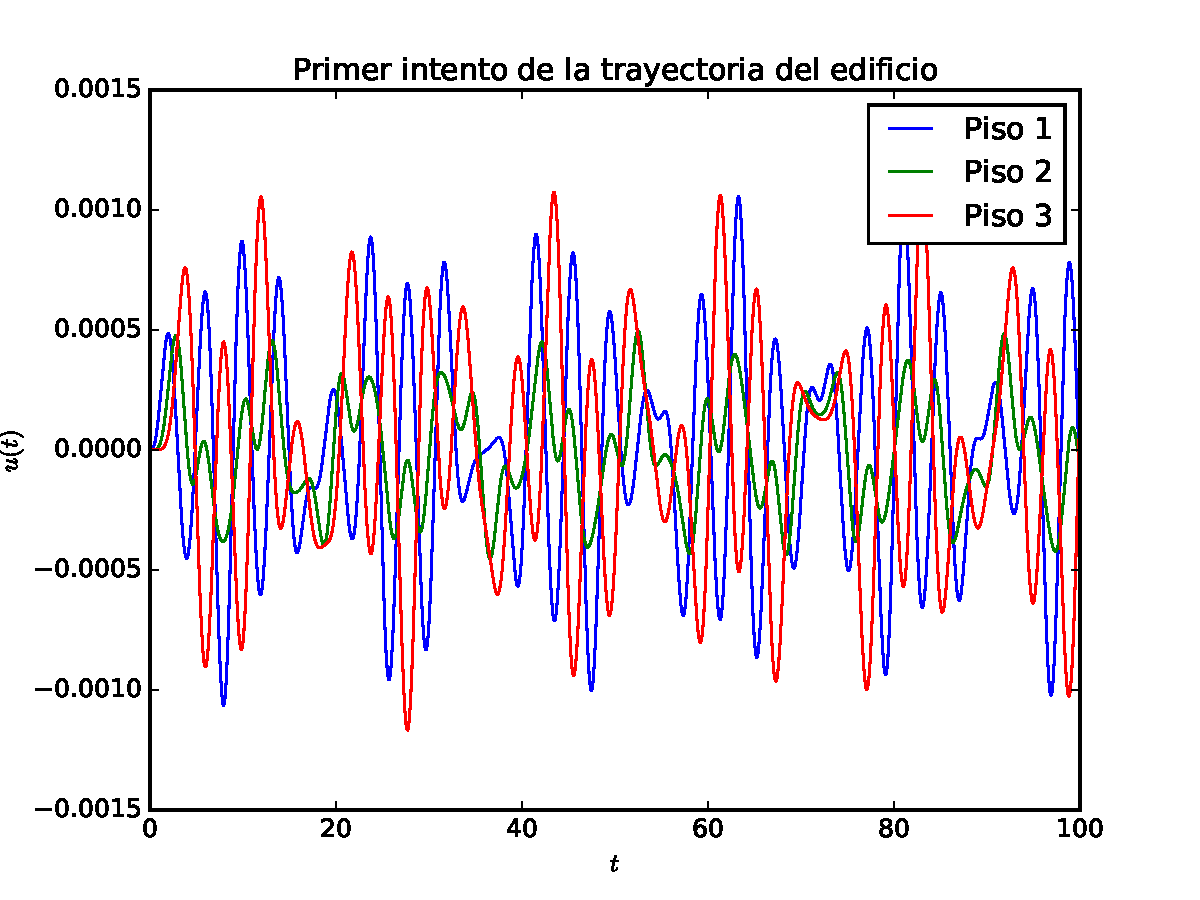
\includegraphics[width=14cm]{3_PrimerEdificio.pdf}
\end{center}
Gráfica de la trayectoria del centro de masa de cada piso $u_i(t)$ durante un sismo que ejerce una fuerza periódica $F(t)=\sin(\omega t)$ con $\omega=\sqrt{\frac{k}{m}}$ donde $k$ modela la rigidez de la estructura y $m$ la masa de cada piso. Para esta frecuencia en particular los pisos 1 y 3 oscilan con mayor amplitud que el segundo piso, que parece más estable.
\begin{center}
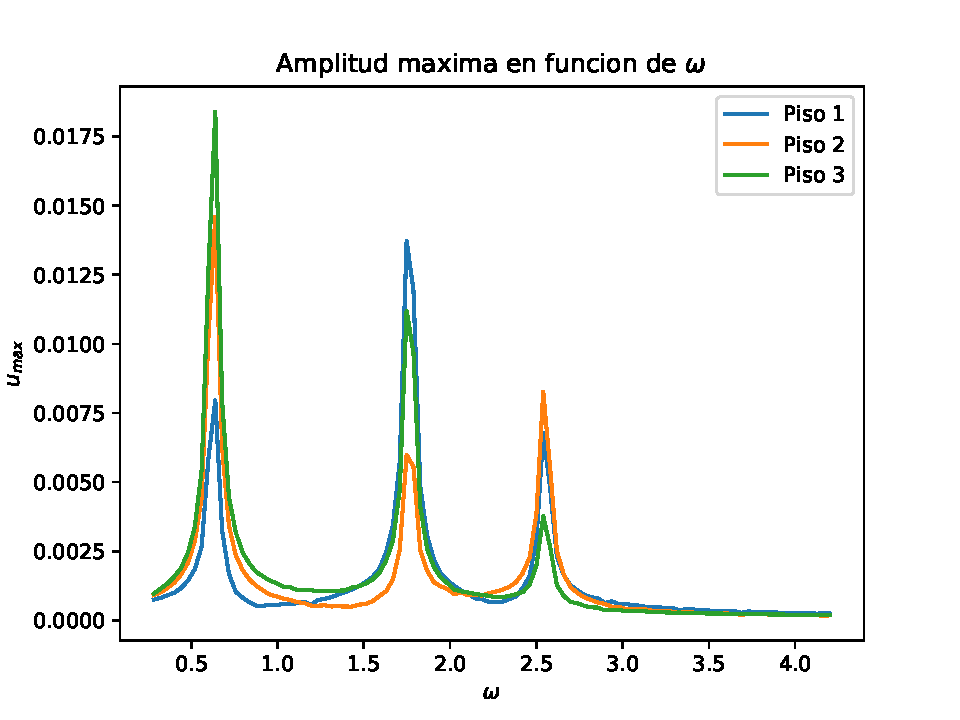
\includegraphics[width=14cm]{3_Maximos.pdf}
\end{center}
Gráfica de la amplitud máxima de la oscilación $u_{max}$ de cada piso en función de la frecuencia del sismo $\omega$ en el intervalo $\left[0.2\sqrt{\frac{k}{m}},3\sqrt{\frac{k}{m}} \right]$. Se pueden ver claramente tres picos, las cuales corresponderán a un tipo particular de resonancia del edificio. Usando Python podemos ver que las frecuencias para las cuales hay resonancia son $\omega_1=0.639225$, $\omega_2=1.74797$ y $\omega_3=2.53993$. Estas frecuencias me parecen las más interesantes pues permiten ver el comportamiento de la estructura en su límite, es decir, cuando el terremoto resuena la misma.
\begin{center}
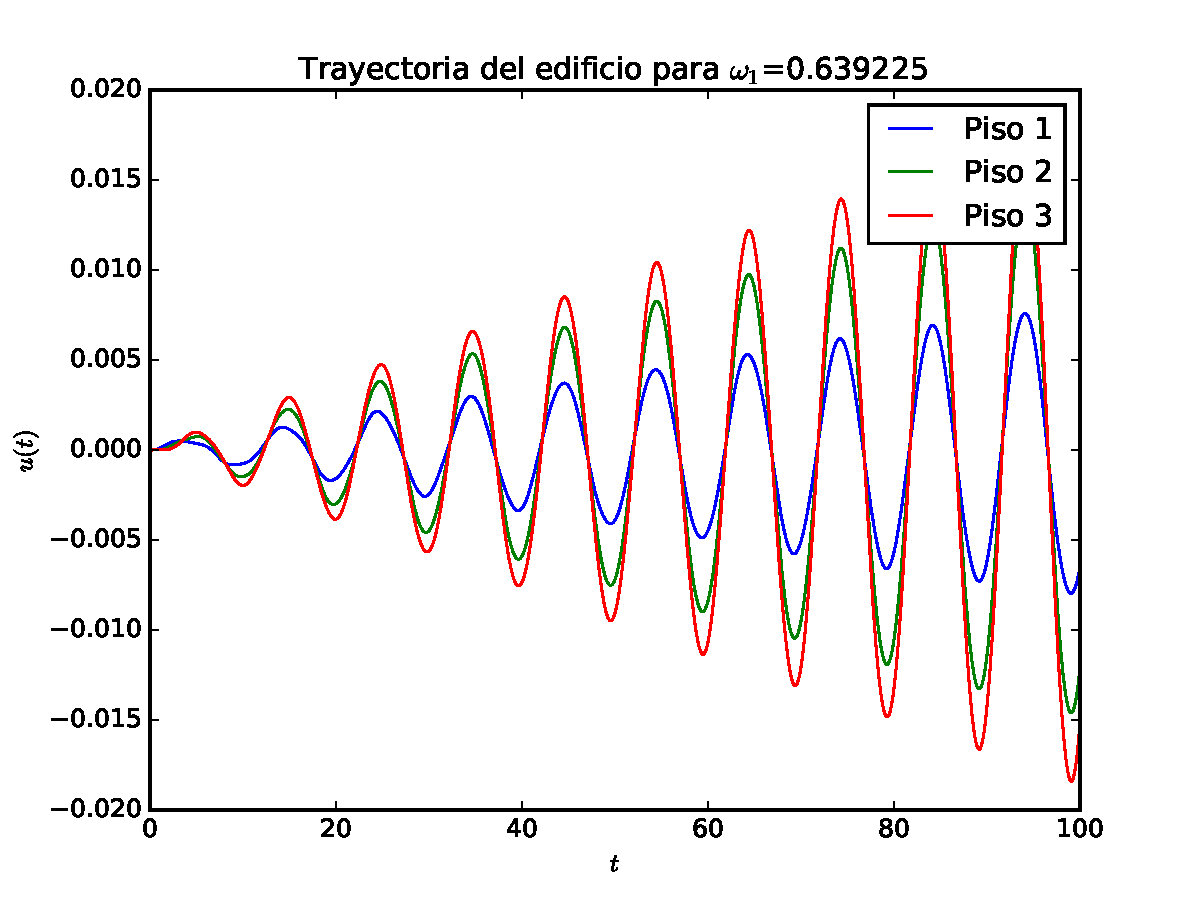
\includegraphics[width=14cm]{3_Edificio_omega1.pdf}
\end{center}
El primer tipo de resonancia hace que el tercer piso tenga la mayor amplitud de oscilación, de hecho la amplitud más grande de todas las frecuencias. Aquí el tercer piso 'domina' el movimiento, haciendo que los otros dos pisos sigan tras él. En una situación realista, se podría especular, éste es el caso muy peligroso, pues que todos los pisos oscilen en la misma dirección con alta amplitud puede hacer que la estructura colapse.
\begin{center}
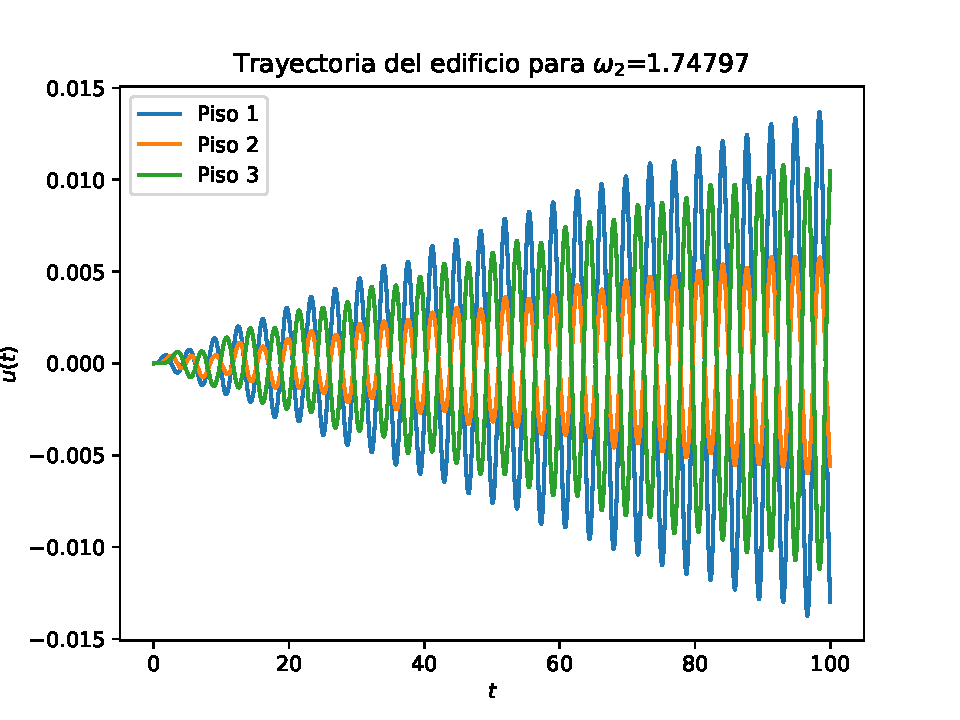
\includegraphics[width=14cm]{3_Edificio_omega2.pdf}
\end{center}
El tercer piso de resonancia hace que el primer piso tenga la mayor amplitud de oscilación. El segundo piso no cambia fuertemente, pero el tercer piso oscila con una amplitud similar a la del primer piso. Esta situación es particularmente peligrosa, pues la estructura del edificio se puede ver comprometida por la gran tensión que siente el piso medio.
\begin{center}
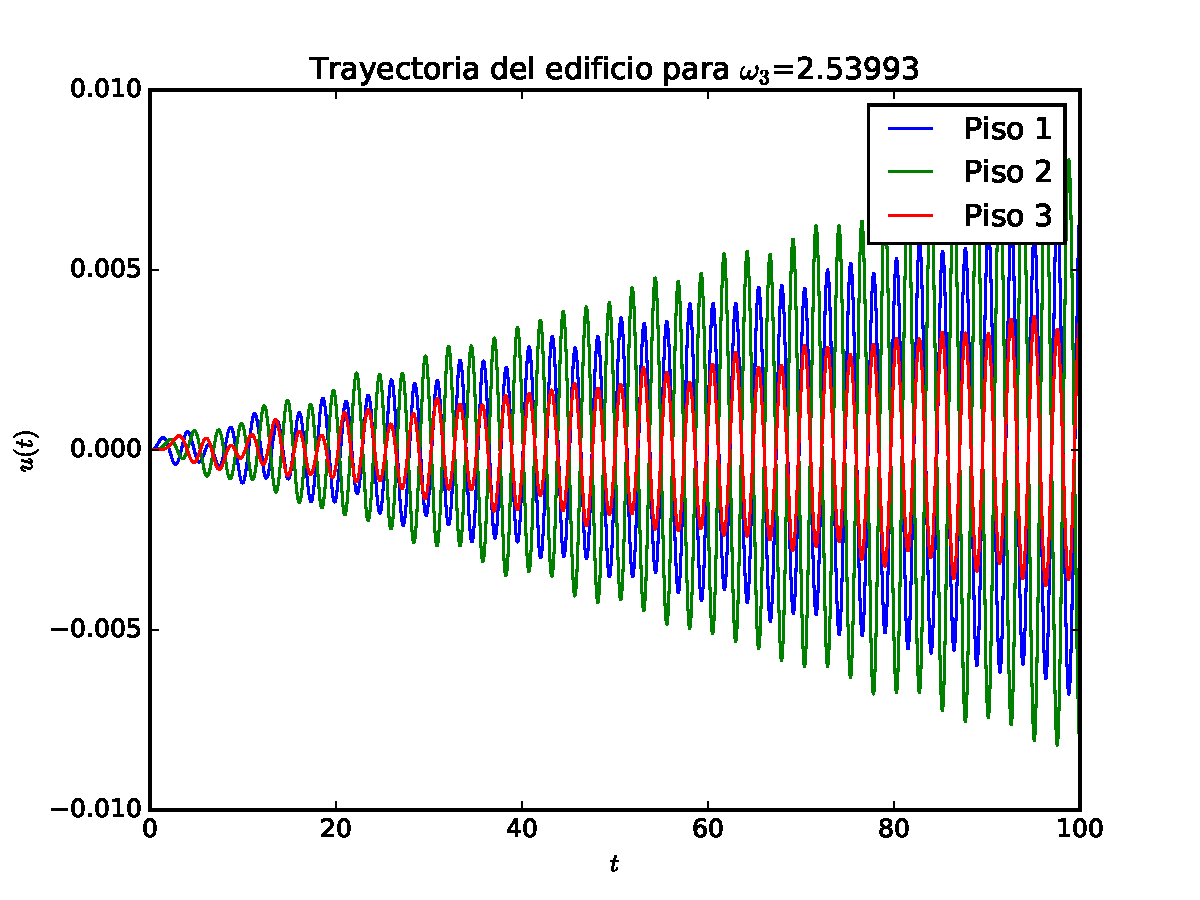
\includegraphics[width=14cm]{3_Edificio_omega3.pdf}
\end{center}
El tercer tipo de resonancia hace que el segundo piso tenga la mayor amplitud. Los otros dos pisos se mueven en la dirección contraria al segundo. Al igual que el caso anterior, esta situación es peligrosa, pues la estructura se deforma alrededor del segundo piso.
\end{document}
